\parindent=0em
\subsection{HP VR1000-127il}
\noindent

Este \textit{HMD} de la empresa \textit{HP} salió al mercado en el año 2018, es un dispositivo dependiente de un ordenador compatible con la plataforma \textit{Windows Mixed Reality}. Este casco se conecta a dicho ordenador a través de una conexión 2 en 1 que combina un \textit{HDMI} 2.0 y \textit{USB} 3.0. \\

Las gafas \textit{HP VR1000-123il} (figura~\ref{fig:hpvr1000}) utilizan dos controladores inalámbricos (que se conectan mediante \textit{bluetooth}) para controlar el movimiento de las manos, estos controladores utilizan 2 pilas AA cada uno. El dispositivo tiene un campo de visión de 90º y una resolución de 1.440×1.440 píxeles por ojo (un total de 2.880x1.440 píxeles con ambos ojos), por otro lado, el casco cuenta con \textit{6DoF} y la \textit{IPD} no se puede regular. 

\begin{figure}[H]
    \centering
    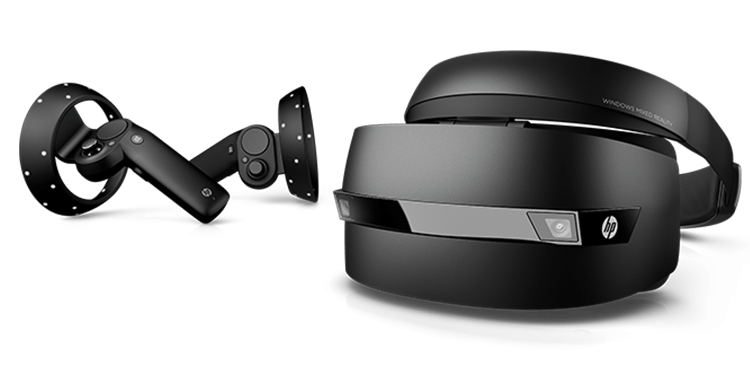
\includegraphics[scale=0.45]{Images/Estado del arte/HP VR1000.png}
    \caption{HP VR1000-123il y sus controladores.}
    \label{fig:hpvr1000}
\end{figure}

Finalmente, este \textit{HMD} no tiene un diseño centrado en su uso con gafas y tiene un peso de 834 gramos. 